\chapter{Stima dell'assetto tramite sensor fusion (NON completo)}
\label{elaborazione}
In questo capitolo vengono inizialmente illustrati gli strumenti matematici utilizzati per rappresentare l'assetto di un corpo rigido nello spazio,
successivamente viene illustrato l'algoritmo di fusione dei dati, provenienti dall'unità di misura inerziale, utilizzato per la stima dell'assetto dell'operatore.


\section{Rappresentazione geometrica dell'assetto di un corpo rigido nello spazio}
\label{assetto}
Con \textit{"assetto di un corpo rigido"} si intende l'orientamento di un corpo rigido rispetto ad un particolare sistema di riferimento.\\
Tale orientamento è rappresentato da una matrice di rotazione che, applicata ad un qualsiasi vettore nel sistema di riferimento mobile, ne fornisce una rappresentazione nel sistema di riferimento fisso (\ref{modello_di_misura}). 
Tale rotazione può essere espressa attraverso numerosi strumenti matematici, tra i più utilizzati si hanno:
\begin{itemize}
	\item \textbf{Angoli di Eulero}
	\item \textbf{Quaternioni unitari}
\end{itemize}

Nella Tab.\ref{rappresentazioni} vengono riportate sinteticamente le caratteristiche delle rappresentazioni appena enunciate \cite{assetto}:

\begin{table}[H]
	\centering

	\label{rappresentazioni}
	\begin{tabular}{lllll}
		\cline{1-3}
		\multicolumn{1}{|l|}{\textbf{Rappresentazione}} & \multicolumn{1}{l|}{\textbf{\#Parametri}} & \multicolumn{1}{l|}{\textbf{Caratteristiche}}                                                                                                                                                                                                                                                    &  &  \\ \cline{1-3}
		\multicolumn{1}{|l|}{Angoli di Eulero}          & \multicolumn{1}{c|}{3}                    & \multicolumn{1}{l|}{\begin{tabular}[c]{@{}l@{}}- facilmente interpretabili \\ dall'essere umano\\ \\ - funzioni trigonometriche nelle \\ relazioni cinematiche\\ \\ -soffrono del fenomeno \\ noto come \textit{Gimbal lock}\\ \\ - meno accurati dei quaternioni\end{tabular}}                           &  &  \\ \cline{1-3}
		\multicolumn{1}{|l|}{Quaternioni unitari}       & \multicolumn{1}{c|}{4}                    & \multicolumn{1}{l|}{\begin{tabular}[c]{@{}l@{}}- non interpretabili facilmente\\ dall'essere umano\\ \\ - equazioni della cinematica \\ lineari\\ \\ - costo computazione di \\ elaborazione minore degli\\ angoli di Eulero\\ \\ - necessitano di un vincolo di \\ norma unitaria\end{tabular}} &  &  \\ \cline{1-3}
		&                                           &                                                                                                                                                                                                                                                                                                  &  & 
	\end{tabular}
	\caption{Tabella comparativa delle rappresentazioni d’assetto}
\end{table}
Nell'algoritmo di fusione dei dati, dettagliato nei paragrafi successivi, si è adottato un approccio ibrido molto comune nei contesti applicativi dei sistemi IPS(\ref{IPS}). Tale approccio consiste nell'utilizzare la rappresentazione mediante \textit{quaternioni} per le computazioni mentre la rappresentazione mediante gli \textit{angoli di Eulero} per la visualizzazione.\\

\subsection{Matrice di rotazione}
Di seguito si fornisce una definizione generale di matrice di assetto\cite{assetto2}. Si supponga di avere due sistemi di riferimento cartesiani in tre dimensioni $F$ e $G$, una matrice ortogonale $A_{FG}$, detta di rotazione ed un vettore $x_G$ espresso nel sistema di riferimento $G$.\\
La matrice $A_{FG}$ permette di esprimere il vettore $x_G$ rispetto al sistema di riferimento $F$ secondo la seguente equazione:

\begin{equation}
x_F = A_{FG}x_G
\end{equation}
Essendo per ipotesi la matrice $A_{FG}$ ortogonale, l'operazione di inversione corrisponde al calcolo della sua trasposta:
 \begin{equation}
 x_G = A_{FG}^Tx_F
 \end{equation}
 Quindi determinare l'assetto significa definire la matrice di rotazione che permette, attraverso una semplice moltiplicazione, di ruotare i vettori da un sistema di riferimento mobile ad uno fisso.\\
 

\subsection{Angoli di Eulero}
Si consideri \cite{assetto2} un sistema di riferimento cartesiano $F$  fisso (con assi $x_F$,$y_F$ e $z_F$) ed un sistema di riferimento cartesiano $G$ mobile (con assi $x_G$,$y_G$ e $z_G$). \\
Affinché l'orientamento degli assi del sistema mobile $G$ coincida con quelli del sistema fisso $F$, si devono eseguire almeno tre rotazioni successive attorno ai tre assi.\\
Tale vincolo è posto dal teorema di Eulero che è alla base di tutte le matrici di rotazioni. Il teorema afferma che:
\begin{itemize}
	\item Per ogni rotazione, esiste sempre un vettore che avrà la medesima rappresentazione nei due sistemi di riferimento
	\item ogni rotazione avviene sempre attorno ad un asse fisso
\end{itemize} 
L'idea è quella di ruotare ogni volta il sistema attorno ad uno dei suoi tre assi, così facendo l'asse attorno al quale è avvenuta la rotazione rimane fisso, mentre gli altri due cambiano orientamento. La rotazione successiva verrà fatta attorno ad uno dei due precedenti assi che hanno mutato l'orientamento. Con sistemi cartesiani a tre assi è possibile quindi scegliere tra dodici differenti sequenze di rotazioni per un totale eguale di possibili rappresentazioni della matrice di rotazione.\\
Nell'ambito di questa tesi e più comunemente in quello aeronautico, si è utilizzata la sequenza di rotazioni $z$-$y$-$x$ e gli angoli $\psi$,$\vartheta$ e $\varphi$ chiamati rispettivamente \textit{imbardata,beccheggio e rollio} (in inglese \textit{yaw,pitch e roll}) mostrati in Fig.\ref{fig:rpy}:
\begin{figure}[H]  
	\centering 
	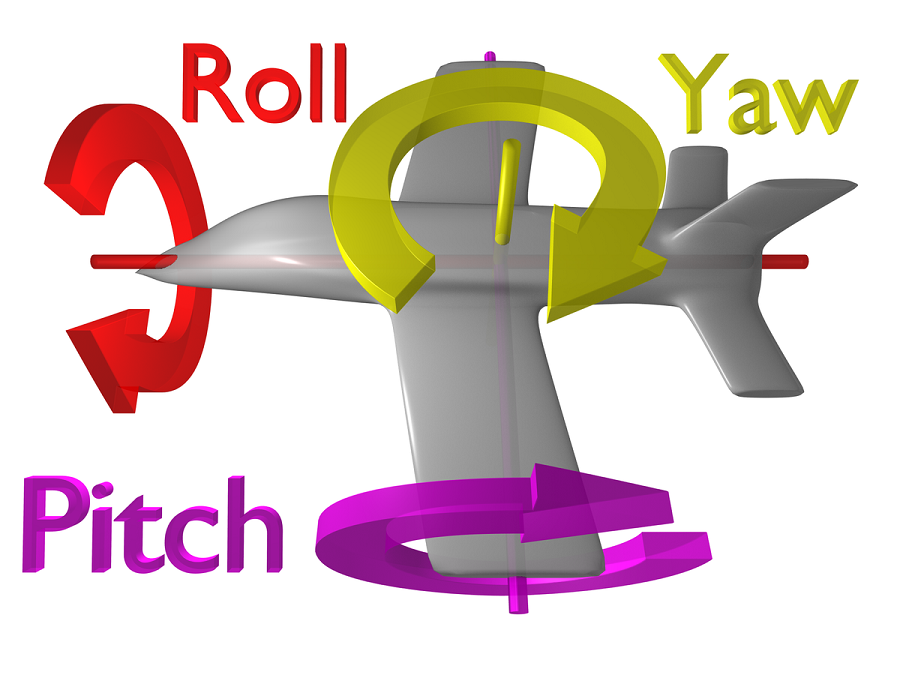
\includegraphics[scale=0.5]{elaborazione/rpy.png}
	\caption{Rappresentazione degli angoli di roll, pitch e yaw per un velivolo \cite{wikiRoll}}
	\label{fig:rpy}
\end{figure}
Le tre rotazioni in questione sono:

\begin{equation}
A(z,\psi)= \begin{bmatrix}
\cos\psi   &-\sin\psi & 0 \\
\sin\psi     & \cos\psi  & 0 \\
0      & 0 & 1
\end{bmatrix}
\end{equation}

\begin{equation}
A(y,\vartheta)= \begin{bmatrix}
\cos\vartheta   &0 & \sin\vartheta \\
0    & 1  & 0 \\
-\sin\vartheta     & 0 & \cos\vartheta
\end{bmatrix}
\end{equation}


\begin{equation}
A(x,\varphi)= \begin{bmatrix}
1   &0 & 0 \\
0    & \cos\varphi  & -\sin\varphi\\
0     & \sin\varphi & \cos\varphi
\end{bmatrix}
\end{equation}

Andando a moltiplicare le precedenti matrici si ottiene la matrice di rotazione cercata:

\begin{eqnarray}
\label{matriceRotazione}
A(\psi,\vartheta,\varphi)= \begin{bmatrix}
\cos\psi \cos\vartheta  & \cos\psi \sin\vartheta \sin\varphi-\sin\psi \cos\varphi & \cos\psi \sin\vartheta \cos\varphi + \sin\psi \sin\varphi \\
\sin\psi \cos\vartheta    & \sin\psi \sin\vartheta \sin\varphi+\cos\psi \cos\varphi & \sin\psi \sin\vartheta \sin\varphi - \cos\psi \sin\varphi\\
-\sin\vartheta    & \cos\vartheta\sin\varphi & \cos\vartheta\cos\varphi
\end{bmatrix}
\end{eqnarray}

Il significato geometrico si ha osservando la Fig.\ref{fig:eulero}, dove:
\begin{itemize}
	\item la linea dei nodi è definita come l'intersezione tra il piano individuato dagli assi $x_Fy_F$ e quello individuato dagli assi $y_Bz_B$
	\item $\psi$ è l'angolo tra $y_F$ e la linea dei nodi
	\item $\vartheta$ è l'angolo tra $x_B$ e la sua proiezione sul piano $x_Fy_F$
	\item $\varphi$ è l'angolo tra $y_B$ e la linea dei nodi
\end{itemize}

\begin{figure}[H]  
	\centering 
	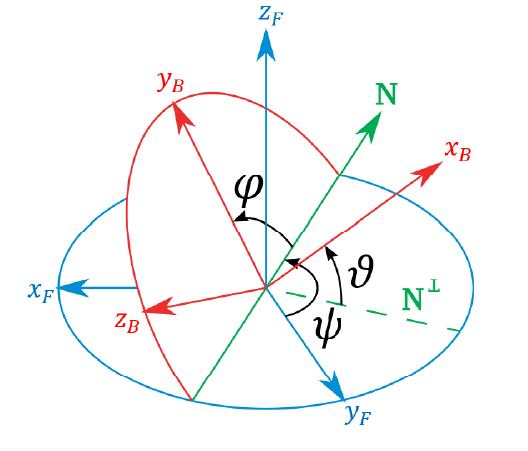
\includegraphics[scale=0.8]{elaborazione/eulero.png}
	\caption{Significato geometrico degli angoli di Eulero \cite{assetto2}}
	\label{fig:eulero}
\end{figure}
Come accennato nella tabella \ref{rappresentazioni}, la rappresentazione dell'assetto mediante angoli di Eulero presenta un problema di singolarità noto come \textit{gimbal lock}.\\
Nel caso della matrice di rotazione ricavata nell'equazione \ref{matriceRotazione}, il problema si presenta per $\vartheta = \pm \dfrac{\pi}{2}$: in questa situazione esistono infinite combinazioni di $\varphi$ e $\psi$ che portano alla stessa matrice di rotazione, nel caso di $\vartheta= \dfrac{\pi}{2}$ si ha:
\begin{equation}
\label{matriceGimbal}
A(\psi,\vartheta,\varphi)= \begin{bmatrix}
0   &\sin(\varphi - \psi) & \cos(\varphi - \psi) \\
0    & \cos(\varphi-\psi)  &-\sin(\varphi - \psi)\\
-1    & 0 & 0
\end{bmatrix}
\end{equation}
Ottenuta mediante sostituzione e applicazione delle formule di addizione e sottrazione di seno e coseno. Mentre la matrice di rotazione in Eq.\ref{matriceRotazione} permette una rotazione completa attorno ad un qualsiasi asse, la matrice in \ref{matriceGimbal} permette la rotazione attorno al solo asse $X$. Quindi si manifesta un vincolo di rotazione con conseguente perdita di un grado di libertà, come mostrato in Fig.\ref{fig:gimbal}. \\
Basti pensare ad un velivolo con un \textit{pitch} di $90°$, modificare il \textit{roll} o lo \textit{yaw} di un certo angolo avrebbe il medesimo effetto.\\
\begin{figure}[H]  
	\centering 
	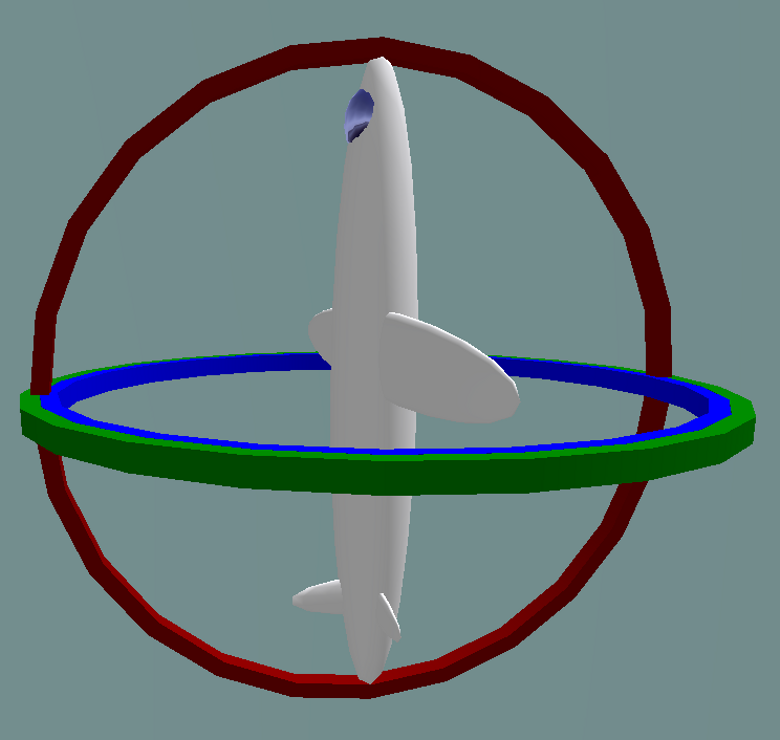
\includegraphics[scale=0.3]{elaborazione/gimbal.png}
	\caption{Rappresentazione del fenomeno di \textit{gimbal lock} \cite{gimbal}}
	\label{fig:gimbal}
\end{figure}



\subsection{Quaternioni unitari}
I quaternioni hanno la peculiarità di essere il metodo di rappresentazione dell'assetto con minor numero di parametri privi di singolarità, come ad esempio il \textit{gimbal lock} visto precedentemente per gli angoli di Eulero.\\
Il quaternione unitario è un vettore composto da tre elementi che definiscono il vettore \textbf{$q_{1:3}$} e da un elemento scalare $q_4$, tale che la norma:
\begin{equation}
 ||\overrightarrow{q}|| = \sqrt{q_1^2 + q_2^2 + q_3^2 + q_4^2}=1
\end{equation}
Questi possono essere usati per rappresentare l'assetto di un corpo rigido in quanto le trasformazioni che legano le terne di Eulero ai quaternioni unitari, sono semplicemente delle trasformazioni algebriche che portano da uno spazio rappresentativo all'altro.\\
Sfruttando il teorema di Eulero \cite{assetto2}, si può parametrizzare la matrice di rotazione in \ref{matriceRotazione} ottenendo l'equivalente in funzione dei quaternioni:
\begin{equation}
\label{matriceQuaternioni}
A(\overrightarrow{q})= \begin{bmatrix}
 q_1^2 -  q_2^2 -  q_3^2 -  q_4^2 & 2(q_1 q_2 + q_3  q_4) & 2(q_1 q_3 - q_2 q_4) \\
2(q_2 q_1 - q_3 q_4)    &  -q_1^2 + q_2^2 -  q_3^2 +  q_4^2  & 2(q_2 q_3 + q_1q_4)\\
2(q_3 q_1 + q_2 q_4)    & 2(q_3 q_2 - q_1 q_4)  &  -q_1^2 -  q_2^2 +  q_3^2 +  q_4^2
\end{bmatrix}
\end{equation}
Come si può notare dalla \ref{matriceRotazione}, i quaternioni permettono di definire una matrice di assetto i cui elementi sono funzioni quadratiche omogenee degli elementi del quaternione. Si evita così qualsiasi tipo di calcolo trigonometrico (e relative singolarità) e si ha un costo computazionale minore.\\

Un diretto confronto tra le matrici \ref{matriceRotazione} e \ref{matriceQuaternioni} permette inoltre di definire il rapporto tra gli angoli di Eulero ($\psi,\vartheta,\varphi$) e le componenti del quaternione ($q_1, q_2, q_3,q_4$) attraverso le seguenti:

\begin{equation}
\psi = Atan2 \left( \frac{2q_2q_3 - 2q_1q_4}{2q_1^2+q_2^2 -1}\right)
\end{equation}

\begin{equation}
\vartheta = -\sin(2q_2q_4 + 2q_1q_3)
\end{equation}

\begin{equation}
\psi = Atan2\left(  \frac{2q_3 q_4 - 2q_1q_2}{2q_1^2+q_4^2 -1}\right)
\end{equation}


\section{Sensor fusion mediante  filtro di Kalman}
\label{sensor_fusion}